\documentclass[border=6pt]{standalone}
\usepackage[T1]{fontenc}
\usepackage{lmodern}
\usepackage{amssymb}
\usepackage{array}
\usepackage{tikz}
\usetikzlibrary{arrows.meta,calc}
\usepackage{pgfplots}
\pgfplotsset{compat=1.18}
\definecolor{cardblue}{HTML}{114d95}
\definecolor{oldorange}{HTML}{7d1f1b}
\definecolor{aqua}{HTML}{deb520}
\definecolor{notsure}{HTML}{A8A69E}
\newcommand{\pieslice}[4]{%
  \fill[#3, draw=white, line width=1.2pt] (0,0) -- (#1:\R) arc[start angle=#1, end angle=#2, radius=\R] -- cycle;
  \node[font=\small\bfseries, text=white] at ({(#1+#2)/2}:{0.62*\R}) {#4};}
\begin{document}
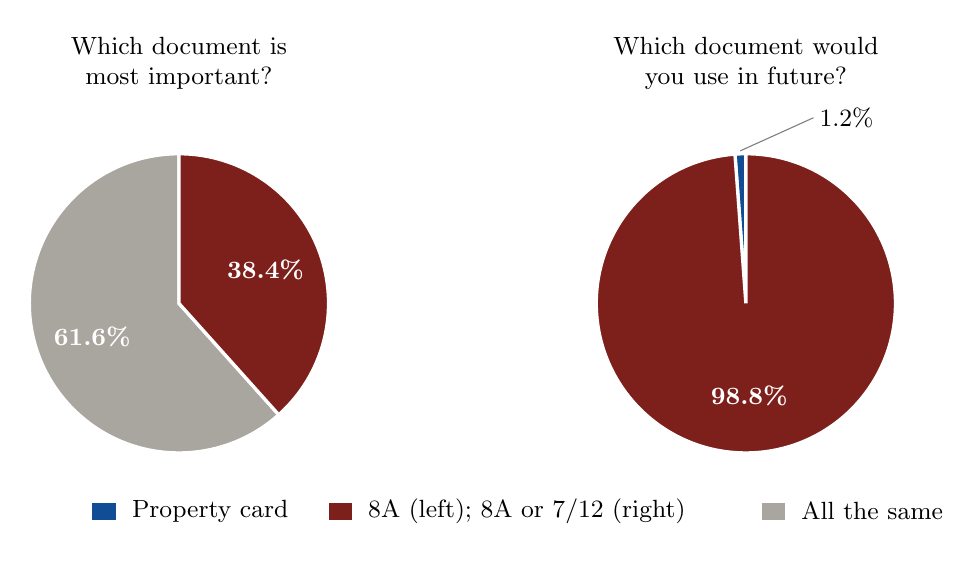
\begin{tikzpicture}
  \def\R{1.9}
  \begin{scope}
    \pieslice{90}{311.86}{notsure}{61.6\%}
    \pieslice{311.86}{450}{oldorange}{38.4\%}
    \node[font=\small, align=center] at (0,3.05) {Which document is\\most important?};
  \end{scope}
  \begin{scope}[xshift=7.2cm]
    \pieslice{90}{94.19}{cardblue}{}
    \pieslice{94.19}{450}{oldorange}{98.8\%}
    \draw[black!50] (92.1:1.02*\R) -- (70:1.32*\R) node[anchor=west, font=\small, text=black, inner sep=2pt] {1.2\%};
    \node[font=\small, align=center] at (0,3.05) {Which document would\\you use in future?};
  \end{scope}
  \begin{scope}[yshift=-2.75cm, xshift=-1.1cm, font=\small]
    \fill[cardblue]  (0,0) rectangle (0.3,0.22);   \node[anchor=west] at (0.38,0.11) {Property card};
    \fill[oldorange] (3.0,0) rectangle (3.3,0.22); \node[anchor=west] at (3.38,0.11) {8A (left); 8A or 7/12 (right)};
    \fill[notsure]   (8.5,0) rectangle (8.8,0.22); \node[anchor=west] at (8.88,0.11) {All the same};
  \end{scope}
\end{tikzpicture}
\end{document}
